\documentclass[10pt,a4paper]{article}
\usepackage[utf8]{inputenc}
\usepackage[spanish]{babel}
\usepackage{amsmath}
\usepackage{amsfonts}
\usepackage{amssymb}
\usepackage{makeidx}
\usepackage{graphicx}
\usepackage{lmodern}
\usepackage{kpfonts}
\usepackage{fourier}
\usepackage[hidelinks]{hyperref}
\usepackage[left=2cm,right=2cm,top=2cm,bottom=2cm]{geometry}
\author{Luis Angel Torres Pinto.\\Universidad Politécnica de la Zona Metropolitana de Guadalajara\\Ingeniería Mecatrónica. }
\title{Explicar los arreglos y parámetros de los Amplificadores Clase B}
\begin{document}
\maketitle
\centering

\includegraphics[scale=1.80]{upzmg.jpg}\\ 
\raggedright
\newpage
\section{Amplificadores clase B}
\part{Caracteristicas y Funcionamiento }
Amplificadores Clase B. Los amplificadores de clase B se caracterizan por tener intensidad casi nula a través de sus transistores cuando no hay señal en la entrada del circuito, por lo que en reposo el consumo es casi nulo.\\
\centering
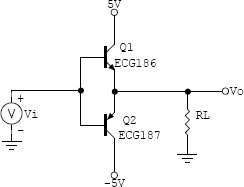
\includegraphics[scale=.90]{Amp.jpg}\\
\raggedright
Un amplificador clase B amplifica un solo semiciclo de la señal de entrada; esto implica situar el punto de trabajo en la región de corte, de tal forma, que sólo al presentarse el semiciclo, el transistor permanece en corte, al igual que en ausencia de señal de entrada.\\
Si se quiere obtener una señal de salida reflejo de la de entrada, se habrán de disponer de forma adecuada, dos transistores, para que cada uno amplifique un semiciclo. Se llama generalmente amplificador de simetria complementaria o push-pull, en la siguiente imagen se muestra;\\
\centering
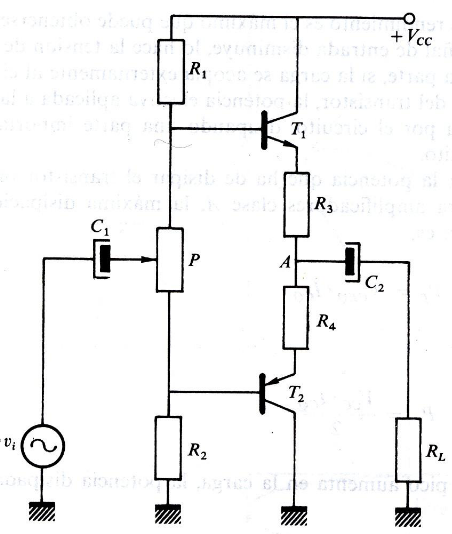
\includegraphics[scale=.40]{b.png}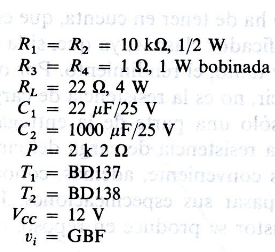
\includegraphics[scale=.60]{bb.png}\\
\raggedright
T1 es NPN y T2 es PNP y, ambos, son compementarios, es decir, presentan iguales características eléctricas, pero de signos opuestos, al ser uno PNP y otro NPN. Se denominan generalmente par complementario o, simplemente, transistores complementarios.\\
La forma básica de alimentar el circuito es disponiendo de una fuente simétrica, que proporciona tensiones +Vcc y -Vcc, conectando la masa o referencia de la fuente a un punto común con vi y RL. Debido a este inconveiente, es más usual el empleo de una sola fuente, haciendo C2 las veces de tal para T2, ya que, como más adelante se verá, cuando este transistor conduzca, queda aislado de +Vcc por que T1 permanece en corte.\\
Al ser C2 de una capacidad elevada (siendo un cortocircuito para la señal de salida), al conducir T1 adquiere carga suficiente a través de T1, R3 y RL; cuando T1 se corta, la tensión en extremos del condensador hace de fuente para T2. Por su elevada capacidad pierde una parte considerablemente pequeña de su carga, que repondrá cuando T1 conduzca de nuevo.
R1, P y R2 componen un divisor de tensión capaz de hacer permanecer a cada transistor en corte, hasta que se aplique vi, cuyos semiciclos positivo y negativo harán conducr a T1 y T2 respectivamente, circulando por RL corriente durante todo el ciclo de vi.\\
Mediante el ajuste de P, se consigue que la tensión entre emisor y colector de cada transistor sea exactamente Vcc/2, con lo que se asegura la igualdad de las polarizaciones de ambos transistores. Este es un modelo simplificado;\\
\centering
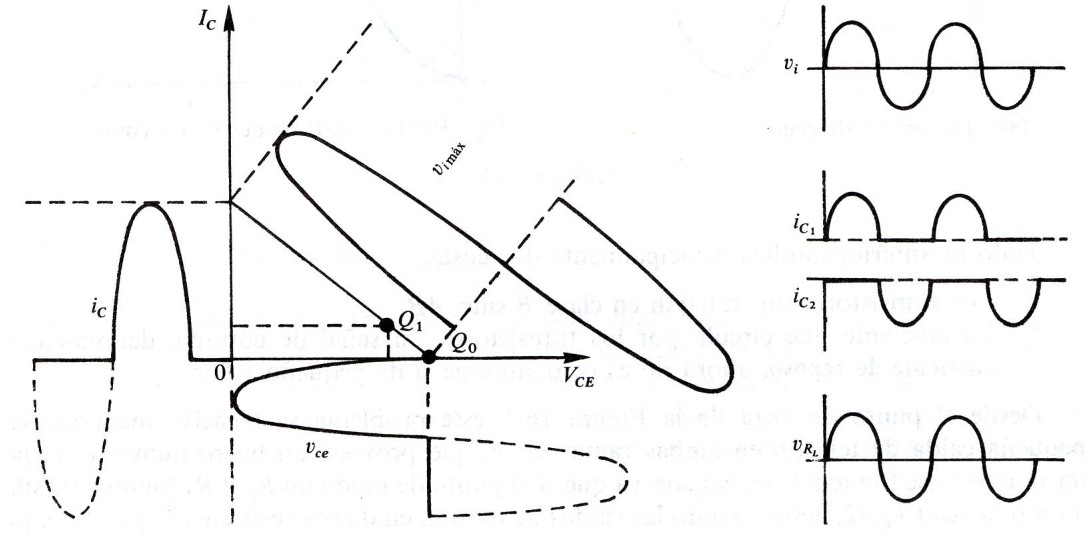
\includegraphics[scale=.40]{gr.png}\\
\centering
Punto de reposo de un amplificador clase B\\
\raggedright
El amplificador de potencia en simetría complementaria presenta un excelente rendimiendo, pues sin señal de entrada el circuito absorbe una corriente mínima y, cuando esta está presente, la mayor parte de la potencia consumida es transferida a la carga.\\
La potencia absorbida de la fuente vendrá determinada por la corriente media en la carga y la tensión de alimentación Vcc (despreciando nuevamente la corriente absorbida por el divisor de polarización de bases R1, P y R2);\\
\centering
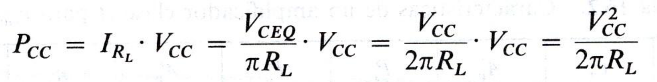
\includegraphics[scale=.50]{for.png}\\
\raggedright
donde IRL es la intensidad media absorbida por la carga.\\
La máxima potencia disipada por la carga se presentará cuando la señal de entrada sea máxima y el punto de trabajo recorra toda la recta de carga, entonces;\\
\centering
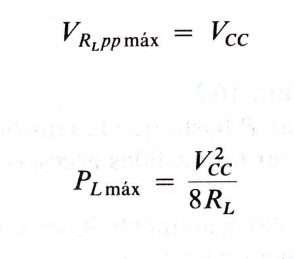
\includegraphics[scale=.60]{Vr.png}\\
\raggedright
\section{Ventajas}
1. Posee bajo consumo en reposo.\\
2. Aprovecha al máximo la Corriente entregada por la fuente.\\
3. Intensidad casi nula cuando está en reposo.\\
\section{Desventajas}
Producen armónicos, y es mayor cuando no tienen los transistores de salida con las mismas características técnicas, debido a esto se les suele polarizar de forma que se les introduce una pequeña polarización directa. Con esto se consigue desplazar las curvas y se disminuye dicha distorsión.
\section{Aplicaciones}
1. Sistemas telefónicos.\\
2. Transmisores de seguridad portátiles.\\
3. Sistemas de aviso, aunque no en audio.\\
\section{Conclusión}
Los amplificadores clase B tienen rendimientos elevados, pero necesitan dos transistores para ofrecer una señal de salida de forma igual a la de entrada. No existe la polarización en amplificador clase B en contra fase cada transistor esta en corte cuando no tiene señal de entrada, lo que resulta una ventaja pues no hay consumo de corriente cuando la señal es cero. La máxima eficiencia en un amplificador clase B en conntrafase es de 78.5\%, por lo que un amplificador de clase B en contrafase se utiliza mas comúnmente como etapa de salida.\\ 
\section{Referencias}
\url{https://www.monografias.com/trabajos89/amplificador-potencia-clase-b/amplificador-potencia-clase-b.shtml}
\url{https://www.ecured.cu/Amplificador_Clase_B}
\url{https://es.scribd.com/doc/139756140/Amplificadores-Clase-b}
\url{https://electronicavm.files.wordpress.com/2011/03/amplificadores-clase-a-y-b1.pdf}
\end{document}